
\chapter{System Implementation}


\section{Hardware Setup}

\subsection{Camera}

\subsection{HD-SDI Interface Card}
The HD-SDI card can be mounted onto a small bracket on the back of the camera. This gives a small 
footprint for the unit. The card is mounted as shown in figure \ref{fig:hd-sdi.card}, where all the connectors are described in 
the figure caption.

The interface has a couple of different functions in the setup. Mainly it does the conversion and 
packing of the LVDS signal from the camera into HD-SDI according to both the HD-SDI protocol and the electrical specification. 
The video data is then available on a MCX7 connector which can be connected to normal BNC using a provided adapter.

There are also a big flat flex cable between the camera and the interface card. This cable is mainly used for sending and receiving the VISCA commands 
to and from the camera. In this situation the interface card provides a level translator so that the signal can be connected directly to a serial 
port on a computer. This serial signal is available on a breakout cable, together with ground references and the analog video outputs from the camera. 

The card also has a single status led to indicate what operating mode the HD-SDI bus is in. On startup the led will be red. This means that 
the video input can not be streamed out to the HD-SDI interface. This usually resolves itself during the setup of the HD-SDI interface between the 
card and the recipient on the other side of the cable. When the setup process is completed, the led will change to green indicating that 
the card is now streaming data. 

During power up, the camera will close and open the iris. This indicates that at least power is getting through. During HD-SDI setup, the camera 
will continue to do this, and it will make clicking sounds. This is a good way of getting feedback without having to constantly 
looking at the interface card.

\begin{figure}
 	\centering
 	\includegraphics[width=0.94\textwidth]{em1571_real}
 	\caption{EM15710 connected to the camera. Blue flat cable on the top is LVDS from camera. Gray flat flex to the left contains 
 		analog HD, communication and power to the camera. Multicolor molex in the bottom middle contains the analog video signals and level translated communication signals. Molex on the top is power. Gold MCX/BNC is HD-SDI out. Status led on the top left corner is red during signal locking and green during normal operation.}
 	\label{fig:hd-sdi.card}
\end{figure}

\subsection{Underwater Housing}\todo{Add better spec}
As the camera needs to be submerged in water, a waterproof housing for the camera was made by the mechanical workshop at the institute. The housing can 
be seen in figure \vref{fig:housing}. The housing is made up of a tube of clear acrylic plastic with two end pieces. The back piece also
has a sliding bracket that the camera can be mounted to. It also has two nipples for the two cables that is going to carry the video signal and 
the power and control signals. 

\begin{figure}
 	\centering
 	\includegraphics[width=0.94\textwidth]{camera_housing}
 	\caption{Underwater housing designed by the Terje Haugen at the mechanical workshop at the institute with camera seated at the holding bracket. Nipples for the 
 		water tight cable connection using a normal 75 $\Omega$ coaxial cable for the video and a Ethernet CAT-5E twisted pair cable for power and serial data.}
 	\label{fig:housing}
\end{figure}
\todo{Add work scetch of housing?}
As seen in figure \ref{fig:housing} the housing also comes with a outer mounting bracket in white acrylic. This is used to attach the housing to the underwater 
part of the rig as described in section \vref{sec:test.rig}. Both the front and back cover of the housing is removable using three screws. To ensure that 
the housing is waterproof there are also a slot on each cover that has a o-ring that gives a tight seal between the inside of the housing and the covers.

\subsection{Underwater Lights}
To mimic the setup from Argus described in \vref{sec:spec.underwater.light}, some cheaper LED based lights were bought. The lights are two casings 
which delivers \SI{27}{\watt}. Each casing has 9 LEDS, each rated to \SI{3}{\watt}. The lights are shown in figure \vref{fig:underwater_light}.

\begin{figure}[htbp]
	\centering
	\includegraphics[width=0.8\textwidth]{led_light}
	\caption{Underwater LED lights mounted on a plywood backing plate}
	\label{fig:underwater_light}
\end{figure}

The lights are originally meant to be mounted on a ships hull to light up the surrounding waters of the boat. 
This means that the lights are designed for mounting on top of a flat surface, which makes things easier for us. It 
is also delivered with a \SI{12}{\volt DC} driver which means that it can be connected to any 
\SI{12}{\volt} source.

\subsection{Cabling}
The cabling used in the test are divided between the video stream and the other cable that provides power and communication with the camera.
The video stream were transferred using a off the shelf 75 $\Omega$ coaxial cable with standard BNC connectors attached to it. This 
connects between the HD-SDI interface and the Ultrastudio SDI unit as depicted in figure \vref{fig:hw.schema}.

The secondary cable used were a CAT5E Ethernet Twisted Pair cable. As this is a cable made from eight pair that is twised in four pairs this 
had enough leads to transport both power and communication. Two of the pairs were used to carry the power to the camera. The last four leads 
were connected to the RX, TX and GND lines on a a USB-RS232 adapter. This meant that the camera could be controlled over a USB port which 
is easier on a modern laptop.

\begin{table}[htbp]
	\centering
	\begin{tabular}{lll}
		\toprule
			HD-SDI Interface 									& CAT5E Cable				& RS232 Adapter \\
		\midrule
			Pin 1, RXD (Brown)									& Green/White				& Pin 3, TX		\\
			Pin 2, TXD (Black)									& Blue						& Pin 2, RX		\\
			Pin 5, GND (Yellow)									& Green						& Pin 5, GND	\\
		\midrule
			Power 1, \SI{9}{\volt} $\pm$ \SI{3}{\volt} (Red)	& Orange \& Orange/White	&				\\
			Power 2 \& 3, GND									& Brown \& Brown/White		&				\\
		\bottomrule
	\end{tabular}
	\caption{Signal cable connections for communication and power}
	\label{tbl:cabeling.connections}
\end{table}


\subsection{Hardware Schematic}
Figure \vref{fig:hw.schema} describes how the different parts of the system interconnects. The figure includes the Ethernet interface in addiditon to the 
HD-SDI interface. The different domains of the system are also shown. This is marked as Local, Transmission and Remote.

Remote in this contex means all the things that are either connected directly to the camera or needs to be within a small distance of the camera. In figure \ref{fig:hw.schema} 
this includes the two interface cards used. Transmission is the part where all the distance between the camera and the recieving computer. Local points at the part 
of the systems that are in close vicinity of the recieving computer. 

Figure \ref{fig:hw.schema} also shows all the different signals and directions of the signals. This in addition to table \vref{tbl:cabeling.connections} should 
give a fairly complete picture of how things are interconnected.

\begin{sidewaysfigure}
	\centering
	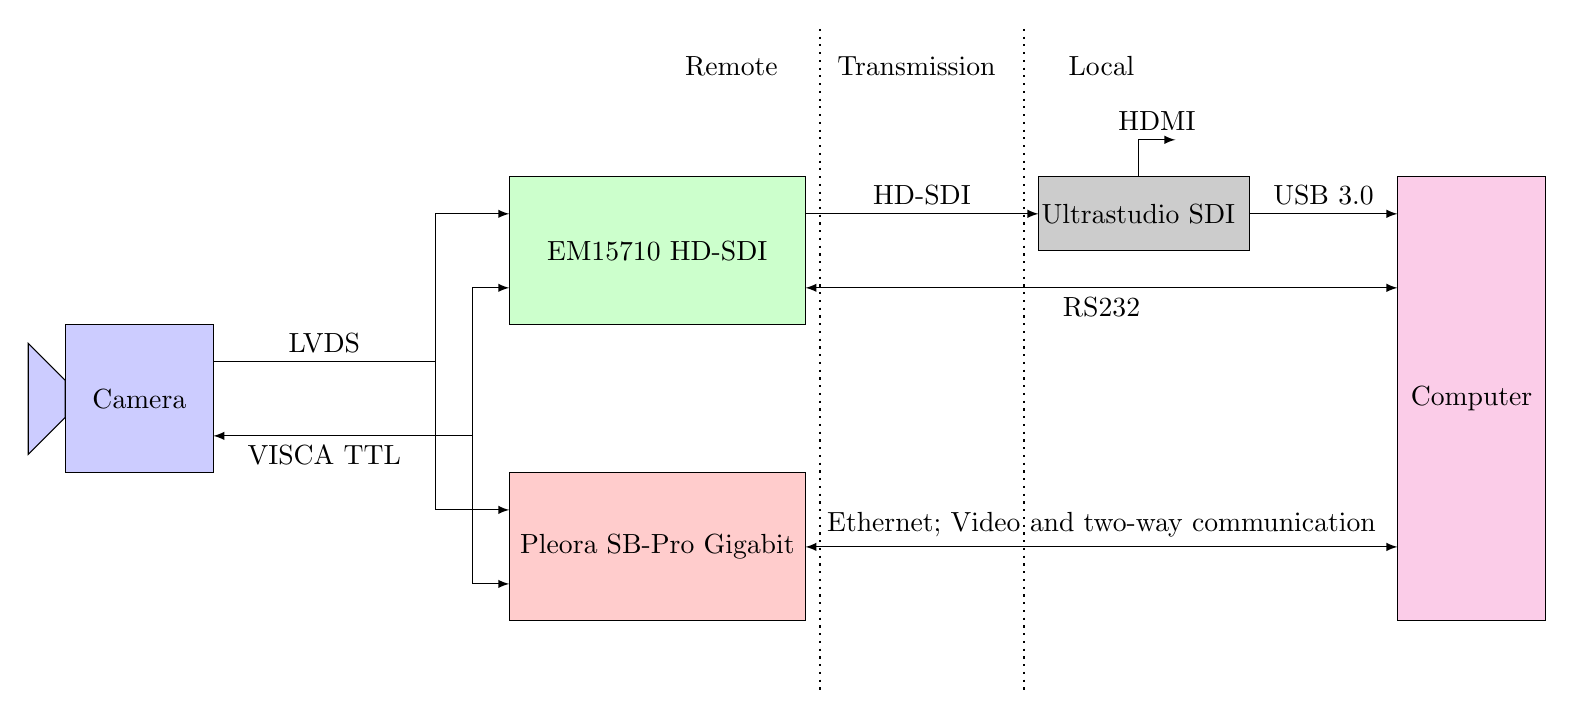
\begin{tikzpicture}[scale=0.94]
		% Camera
		\filldraw[fill=blue!20!white] (0,1) rectangle (2,-1);
		\filldraw[fill=blue!20!white] (0,0.25) -- (-0.5,0.75) -- (-0.5,-0.75) -- (0,-0.25) -- (0,0.25);
		\filldraw[fill=blue!20!white,draw=blue!20!white] (-0.1,-0.25) rectangle (0,.1,0.25);
		\node() at (1,0) {Camera};
		
		% EM
		\filldraw[fill=green!20!white] (6,1) rectangle (10,3);
		\node() at (8, 2) {EM15710 HD-SDI};
		
		% PL
		\filldraw[fill=red!20!white] (6,-1) rectangle (10,-3);
		\node() at (8, -2) {Pleora SB-Pro Gigabit};
		
		% U-SDI
		\filldraw[fill=black!20!white] (13.15,2) rectangle (16,3);
		\node() at (14.5, 2.5) {Ultrastudio SDI};
		
		% PC
		\filldraw[fill=magenta!20!white] (18,-3) rectangle (20,3);
		\node() at (19,0) {Computer};
		
		% Horiz lines
		\draw[thick,dotted] (10.2,5) -- (10.2,-4);
		\draw[thick,dotted] (12.95,5) -- (12.95,-4);
		
		% Top lines
		\node() at (9, 4.5){Remote};
		\node() at (11.5, 4.5){Transmission};
		\node() at (14, 4.5){Local};
		
		% Signal lines from camera
		\draw[] (2, 0.5) -- (5, 0.5) node [midway, above] {LVDS};
		\draw[-latex] (5, -0.5) -- (2, -0.5) node [midway, below] {VISCA TTL};
		
		% Signal lines to EM
		\draw[-latex] (5, 0.5) -- (5, 0.5) -- (5, 2.5) -- (6, 2.5);% LVDS
		\draw[-latex] (5, -0.5) -- (5.5, -0.5) -- (5.5, 1.5) -- (6, 1.5); % TTL
		
		% Signal lines to PL
		\draw[-latex] (5, 0.5) -- (5, 0.5) -- (5, -1.5) -- (6, -1.5); % LVDS
		\draw[-latex] (5, -0.5) -- (5.5, -0.5) -- (5.5, -2.5) -- (6, -2.5); % TTL
		
		% Signal line from EM to U-SDI
		\draw[-latex] (10,2.5) -- (13.15, 2.5) node [midway, above]{HD-SDI};
		
		% Signal line from U-SDI, HDMI
		\draw[-latex] (14.5,3) -- (14.5, 3.5) -- (15, 3.5) node [midway, above]{HDMI};
				
		% Signal line from EM to PC
		\draw[latex-latex] (10,1.5) -- (18, 1.5) node [midway, below]{RS232}; 
		
		% Signal line from U-SDI to PC
		\draw[-latex] (16, 2.5) -- (18, 2.5) node [midway, above]{USB 3.0};
		
		% Signal line from PL to PC
		\draw[latex-latex] (10,-2) -- (18, -2) node [midway, above]{Ethernet; Video and two-way communication}; 
	\end{tikzpicture}
	\caption{Schematics of the hardware, showing both the HD-SDI and the Ethernet pipeline. The different signals and directions are drawn in. 
		Vertical lines express different domains in the system; Remote things on the camera, Transmission for the place where the long distance signals are sent and Local for what is 
		near the computer and the receiving end.}
	\label{fig:hw.schema}
\end{sidewaysfigure}

\subsection{Test Rig}\label{sec:test.rig}

\section{Software}

\subsection{Capture Software}

\subsection{Capture constraints}